\documentclass[11pt,a4paper]{article}

\usepackage[utf8]{inputenc}
\usepackage[T1]{fontenc}
\usepackage[spanish]{babel}
\usepackage{geometry}
\usepackage{graphicx}
\usepackage{array}
\usepackage{tabularx}
\usepackage{makecell}
\usepackage[table]{xcolor}
\usepackage{fancyhdr}
\usepackage{titlesec}
\usepackage{helvet}
\usepackage{ragged2e}
\usepackage{enumitem}
\usepackage{setspace}
\usepackage{hyperref}
\usepackage{booktabs} % Para tablas con acabado profesional
\usepackage{enumitem} % Para control fino de las listas
\usepackage{amsmath}  % Para las fórmulas del modelo

\renewcommand{\familydefault}{\sfdefault}
\geometry{
  a4paper,
  left=3.0cm,
  right=3.0cm,
  top=2.35cm,
  bottom=2.35cm,
  headheight=1.9cm,
  headsep=0.45cm
}

\setlength{\parindent}{0pt}
\setlength{\parskip}{0.22em}
\setlength{\tabcolsep}{6pt}
\renewcommand{\arraystretch}{1.08}

\pagestyle{fancy}
\fancyhf{}
\fancyhead[L]{
\includegraphics[height=1.35cm]{assets/logo_feirnnr.png}}
\fancyhead[R]{\vspace{0.1cm}\small FEIRNNR - Carrera de Computación}
\renewcommand{\headrulewidth}{0.5pt}
\renewcommand{\footrulewidth}{0pt}
\makeatletter
\renewcommand{\headrule}{%
  {\color{gray!65}\hrule width\headwidth height\headrulewidth \vskip-\headrulewidth}%
}
\makeatother

\titleformat{\section}
  {\bfseries\fontsize{15}{17}\selectfont}
  {\thesection.}{0.8em}{}
\titlespacing*{\section}{0pt}{0.7ex}{0.2ex}

\newcolumntype{L}[1]{>{\RaggedRight\arraybackslash}p{#1}}
\newcolumntype{Y}{>{\RaggedRight\arraybackslash}X}

% Marca visible de lo que falta completar (video de demostración).
\newcommand{\pendiente}[1]{\textcolor{red}{\textbf{[PENDIENTE: #1]}}}

% Paleta de las tablas de la plantilla institucional.
\definecolor{headerblue}{RGB}{19, 93, 126}
\definecolor{rowlight}{RGB}{205, 235, 248}
\definecolor{borderblue}{RGB}{64, 160, 206}

\begin{document}
\thispagestyle{fancy}

\vspace*{0.15cm}

\begin{center}
{\bfseries\fontsize{23}{26}\selectfont
Reporte Técnico de Actividades\\
Práctico-Experimentales Nro. 003\par}
\end{center}

\section{Datos de Identificación del Estudiante y la Práctica}

\noindent
\begin{tabularx}{\textwidth}{|L{0.43\textwidth}|Y|}
\hline
\textbf{Nombre del estudiante(s)} & Jaime Alejandro Landázuri Román \\
 & Richard Ariel Chamba Sánchez \\
 & Cael Alejandro Soto Cueva \\
 & Domenica Nicole Rojas Pardo \\ \hline
\textbf{Asignatura} & Simulación \\ \hline
\textbf{Ciclo} & 5 A \\ \hline
\textbf{Unidad} & 1 \\ \hline
\textbf{Resultado de aprendizaje de la unidad} & R1. Aplica análisis estadísticos de los datos
de la Simulación para mejorar la calidad de los resultados, bajo los principios de solidaridad, transparencia, responsabilidad y honestidad. \\ \hline
\textbf{Práctica Nro.} & 003 \\ \hline
\textbf{Título de la Práctica} & Simulación de un sistema de líneas de espera M/M/1 mediante SimPy \\ \hline
\textbf{Nombre del Docente} & José O. Guamán Q. \\ \hline
\textbf{Fecha} & 15 de Octubre de 2026 \\
 & 16 de Octubre 2026 \\ \hline
\textbf{Horario} & Jueves 10h30 a 11h30 \\
 & Viernes 07h30 a 09h30 \\ \hline
\textbf{Lugar} & Aula \\ \hline
\textbf{Tiempo planificado en el Sílabo} & 3 horas \\ \hline
\end{tabularx}

\section{Objetivo(s) de la Práctica}
Simular un sistema de líneas de espera M/M/1 utilizando Python y SimPy, analizando
el comportamiento de los clientes, la cola y el servidor.
\begin{enumerate}
    \item Implementar un modelo M/M/1 utilizando la biblioteca SimPy.
    \item Calcular las principales métricas teóricas del sistema de espera.
    \item Comparar los resultados teóricos con los obtenidos mediante la simulación.
\end{enumerate}

\section{Materiales y reactivos}
\begin{itemize}
    \item Python 3.x.
    \item Biblioteca SimPy.
    \item NumPy.
    \item Matplotlib.
    \item Editor de código: Visual Studio Code, PyCharm o Jupyter Notebook.
\end{itemize}

\section{Equipos y herramientas}
\begin{itemize}
    \item Computador.
    \item Procesador de 2 núcleos o superior.
    \item Mínimo 4 GB de RAM.
    \item Sistema operativo Linux o macOS.
\end{itemize}

\section{Procedimiento / Metodología Ejecutada}

\subsection{Fundamento teórico}

El modelo \textbf{M/M/1} representa un sistema de líneas de espera con llegadas de
clientes siguiendo una distribución de Poisson, tiempos de servicio con distribución
exponencial, un único servidor y atención de clientes bajo el principio FIFO
(\emph{primero en llegar, primero en ser atendido}).

El modelo utiliza dos parámetros principales:
\begin{itemize}
    \item $\lambda$: tasa promedio de llegada de clientes.
    \item $\mu$: tasa promedio de servicio del servidor.
\end{itemize}

La utilización del servidor se calcula mediante:
\[
\rho = \frac{\lambda}{\mu}
\]

\noindent\textbf{Nota sobre una errata de la guía.} La guía de la práctica (§5.1) imprime
$\rho = \mu/\lambda$, lo que contradice su propia condición de estabilidad
$\lambda < \mu$ expresada unas líneas más abajo y también su pseudocódigo, que usa
$\rho = \lambda/\mu$. Con la fórmula impresa, los tres escenarios de la guía darían
$\rho = 1{,}50$, $1{,}20$ y $1{,}03$, es decir un servidor saturado en los tres casos, y
las medidas $L$, $L_q$, $W$ y $W_q$ no existirían (solo están definidas para
$\rho < 1$). Este informe usa la definición correcta $\rho = \lambda/\mu$, que es
además la que aparece en la bibliografía de teoría de colas.

Para que el sistema sea estable debe cumplirse:
\[
\lambda < \mu
\]

Las principales medidas teóricas del sistema son:

\[
L = \frac{\lambda}{\mu-\lambda} \qquad
L_q = \frac{\lambda^2}{\mu(\mu-\lambda)}
\]

\[
W = \frac{1}{\mu-\lambda} \qquad
W_q = \frac{\lambda}{\mu(\mu-\lambda)}
\]

\begin{table}[h!]
\centering
\setlength{\arrayrulewidth}{0.75pt}
\arrayrulecolor{borderblue}
\renewcommand{\arraystretch}{1.25}
\begin{tabular}{|l|l|}
\hline
\rowcolor{headerblue}
\textbf{\textcolor{white}{Símbolo}} & \textbf{\textcolor{white}{Significado}} \\ \hline
$\lambda$ & Tasa de llegada de clientes \\ \hline
\rowcolor{rowlight}
$\mu$ & Tasa de servicio \\ \hline
$\rho$ & Utilización del servidor \\ \hline
\rowcolor{rowlight}
$L$ & Número promedio de clientes en el sistema \\ \hline
$L_q$ & Número promedio de clientes en la cola \\ \hline
\rowcolor{rowlight}
$W$ & Tiempo promedio en el sistema \\ \hline
$W_q$ & Tiempo promedio de espera en la cola \\ \hline
\end{tabular}
\caption{Notación empleada.}
\end{table}

\subsection{Escenarios ejecutados}

Se ejecutaron los tres escenarios indicados por la guía, todos con $\mu = 3{,}0$:

\begin{table}[h!]
\centering
\setlength{\arrayrulewidth}{0.75pt}
\arrayrulecolor{borderblue}
\renewcommand{\arraystretch}{1.25}
\begin{tabular}{|c|c|c|l|}
\hline
\rowcolor{headerblue}
\textbf{\textcolor{white}{Escenario}} & \textbf{\textcolor{white}{$\lambda$}} & \textbf{\textcolor{white}{$\mu$}} & \textbf{\textcolor{white}{Condición}} \\ \hline
1 & 2{,}0 & 3{,}0 & Sistema estable \\ \hline
\rowcolor{rowlight}
2 & 2{,}5 & 3{,}0 & Mayor utilización \\ \hline
3 & 2{,}9 & 3{,}0 & Cerca de saturación \\ \hline
\end{tabular}
\caption{Escenarios de la guía. La utilización teórica resulta $\rho = 0{,}667$,
$0{,}833$ y $0{,}967$ respectivamente.}
\end{table}

\subsection{Implementación}

El programa se desarrolló en Python siguiendo el pseudocódigo de la guía y se
estructuró en tres capas (modelo, vista y controlador) para que cada medida tuviera
un único responsable en el código. Los componentes principales son:

\begin{itemize}
    \item \textbf{Motor de simulación} (\texttt{model/simulation.py}): crea un entorno
    SimPy con un servidor de \texttt{capacity = 1}, genera los clientes con tiempos
    entre llegadas exponenciales de tasa $\lambda$, los atiende en orden FIFO con
    tiempos de servicio exponenciales de tasa $\mu$ y registra, por cada cliente, el
    instante de llegada, el inicio y fin de servicio, el tiempo de espera y el tiempo
    de servicio. El estado del sistema se guarda en un registro inmutable por cliente
    y en una traza de la longitud de la cola a lo largo del tiempo.
    \item \textbf{Métricas teóricas} (\texttt{model/metrics.py}): implementa las
    fórmulas del apartado anterior y actúa como \emph{oráculo} de correctitud del
    simulador.
    \item \textbf{Análisis} (\texttt{model/analysis.py}): agrupa las réplicas por
    escenario, calcula la media simulada, el intervalo de confianza al 95\,\% con la
    distribución $t$ de Student y el error relativo de cada medida frente a la teoría.
    \item \textbf{Tabla y gráficas} (\texttt{view/}): exporta la tabla comparativa a
    CSV y LaTeX, y genera las figuras del informe.
    \item \textbf{Línea de comandos} (\texttt{controller/cli.py}): un solo comando
    reproduce todo el estudio:
\end{itemize}

\begin{verbatim}
python -m mm1 --scenarios --replications 30 --sim-time 1000 --out outputs/
\end{verbatim}

\noindent\textbf{Parámetros de la corrida oficial.} 30 réplicas por escenario,
$\text{sim\_time} = 1000$ unidades de tiempo y semilla base 42, de la cual se derivan
de forma determinista las semillas de cada réplica. En total se ejecutaron
\textbf{90 simulaciones}. La corrida es \textbf{reproducible}: repetir el comando
produce exactamente los mismos números.

\noindent\textbf{Justificación del número de réplicas.} Una sola corrida no es
evidencia suficiente cuando el sistema está cerca de la saturación: con $\rho = 0{,}967$
el tiempo de espera tiene una distribución de cola pesada y una corrida individual
puede desviarse hasta un 74\,\% de la teoría sin que el simulador esté equivocado. Por
eso se promedian 30 réplicas independientes por escenario y se reporta el intervalo de
confianza, que es lo que permite afirmar si la teoría queda o no dentro del rango de lo
simulado.

\section{Resultados}

\subsection{Comparación entre resultados teóricos y simulados}

La Tabla~\ref{tab:comparacion} presenta, para cada escenario, los valores teóricos
obtenidos con las fórmulas del modelo y los valores simulados obtenidos como promedio
de las 30 réplicas.

\begin{table}[h!]
\centering
\setlength{\arrayrulewidth}{0.75pt}
\arrayrulecolor{borderblue}
\renewcommand{\arraystretch}{1.3}
\small
\begin{tabular}{|c|c|c|c|c|c|c|c|c|}
\hline
\rowcolor{headerblue}
\textbf{\textcolor{white}{Esc.}} &
\textbf{\textcolor{white}{$\lambda$}} &
\textbf{\textcolor{white}{$\rho$}} &
\textbf{\textcolor{white}{$L$}} &
\textbf{\textcolor{white}{$L_q$}} &
\textbf{\textcolor{white}{$W$}} &
\textbf{\textcolor{white}{$W_q$}} &
\makecell{\textbf{\textcolor{white}{Espera}} \\ \textbf{\textcolor{white}{simulada}}} &
\makecell{\textbf{\textcolor{white}{Cola}} \\ \textbf{\textcolor{white}{simulada}}} \\ \hline
1 & 2{,}0 & 0{,}6667 & 2{,}0000 & 1{,}3333 & 1{,}0000 & 0{,}6667 & \textbf{0{,}6885} & \textbf{1{,}3921} \\ \hline
\rowcolor{rowlight}
2 & 2{,}5 & 0{,}8333 & 5{,}0000 & 4{,}1667 & 2{,}0000 & 1{,}6667 & \textbf{1{,}6211} & \textbf{4{,}0694} \\ \hline
3 & 2{,}9 & 0{,}9667 & 29{,}0000 & 28{,}0333 & 10{,}0000 & 9{,}6667 & \textbf{8{,}5078} & \textbf{24{,}7945} \\ \hline
\end{tabular}
\caption{Comparación de resultados teóricos y simulados por escenario. Las columnas
$\rho$, $L$, $L_q$, $W$ y $W_q$ son teóricas; las dos últimas son los promedios
simulados de 30 réplicas.}
\label{tab:comparacion}
\end{table}

\subsection{Intervalo de confianza y error relativo}

La Tabla~\ref{tab:intervalos} reporta el intervalo de confianza al 95\,\% de la espera
media simulada y el error relativo de cada medida respecto de su valor teórico. El
intervalo se calculó con la distribución $t$ de Student sobre las 30 medias por réplica,
que es la cantidad que se compara contra la teoría y no la dispersión de clientes
individuales.

\begin{table}[h!]
\centering
\setlength{\arrayrulewidth}{0.75pt}
\arrayrulecolor{borderblue}
\renewcommand{\arraystretch}{1.3}
\small
\begin{tabular}{|c|c|c|c|c|c|c|}
\hline
\rowcolor{headerblue}
\textbf{\textcolor{white}{Esc.}} &
\textbf{\textcolor{white}{Desv. est.}} &
\makecell{\textbf{\textcolor{white}{IC 95\,\% de}} \\ \textbf{\textcolor{white}{la espera}}} &
\makecell{\textbf{\textcolor{white}{\textquestiondown{}Contiene}} \\ \textbf{\textcolor{white}{al teórico?}}} &
\textbf{\textcolor{white}{Err. $L$}} &
\textbf{\textcolor{white}{Err. $L_q$}} &
\textbf{\textcolor{white}{Err. $W_q$}} \\ \hline
1 & 0{,}0983 & $[0{,}6518;\ 0{,}7252]$ & Sí (0{,}6667) & 3{,}19\,\% & 4{,}41\,\% & 3{,}28\,\% \\ \hline
\rowcolor{rowlight}
2 & 0{,}3898 & $[1{,}4755;\ 1{,}7666]$ & Sí (1{,}6667) & 2{,}12\,\% & 2{,}33\,\% & 2{,}73\,\% \\ \hline
3 & 8{,}2631 & $[5{,}4223;\ 11{,}5933]$ & Sí (9{,}6667) & 12{,}69\,\% & 11{,}55\,\% & 11{,}99\,\% \\ \hline
\end{tabular}
\caption{Intervalo de confianza al 95\,\% de la espera media simulada y error relativo
por medida. En los tres escenarios el valor teórico queda \emph{dentro} del intervalo
simulado.}
\label{tab:intervalos}
\end{table}

\noindent\textbf{Hallazgo principal.} En los \textbf{tres} escenarios el valor teórico
de $W_q$ cae dentro del intervalo de confianza al 95\,\% construido con las réplicas
simuladas. Esto significa que el simulador es estadísticamente consistente con el
modelo analítico: las diferencias observadas son compatibles con el error de muestreo y
no con un sesgo de implementación.

\subsection{Gráficas}

La Figura~\ref{fig:teoria} compara teoría y simulación para las cuatro medidas en los
tres escenarios; el panel de $W_q$ incluye el intervalo de confianza como barra de error.

\begin{figure}[h!]
\centering
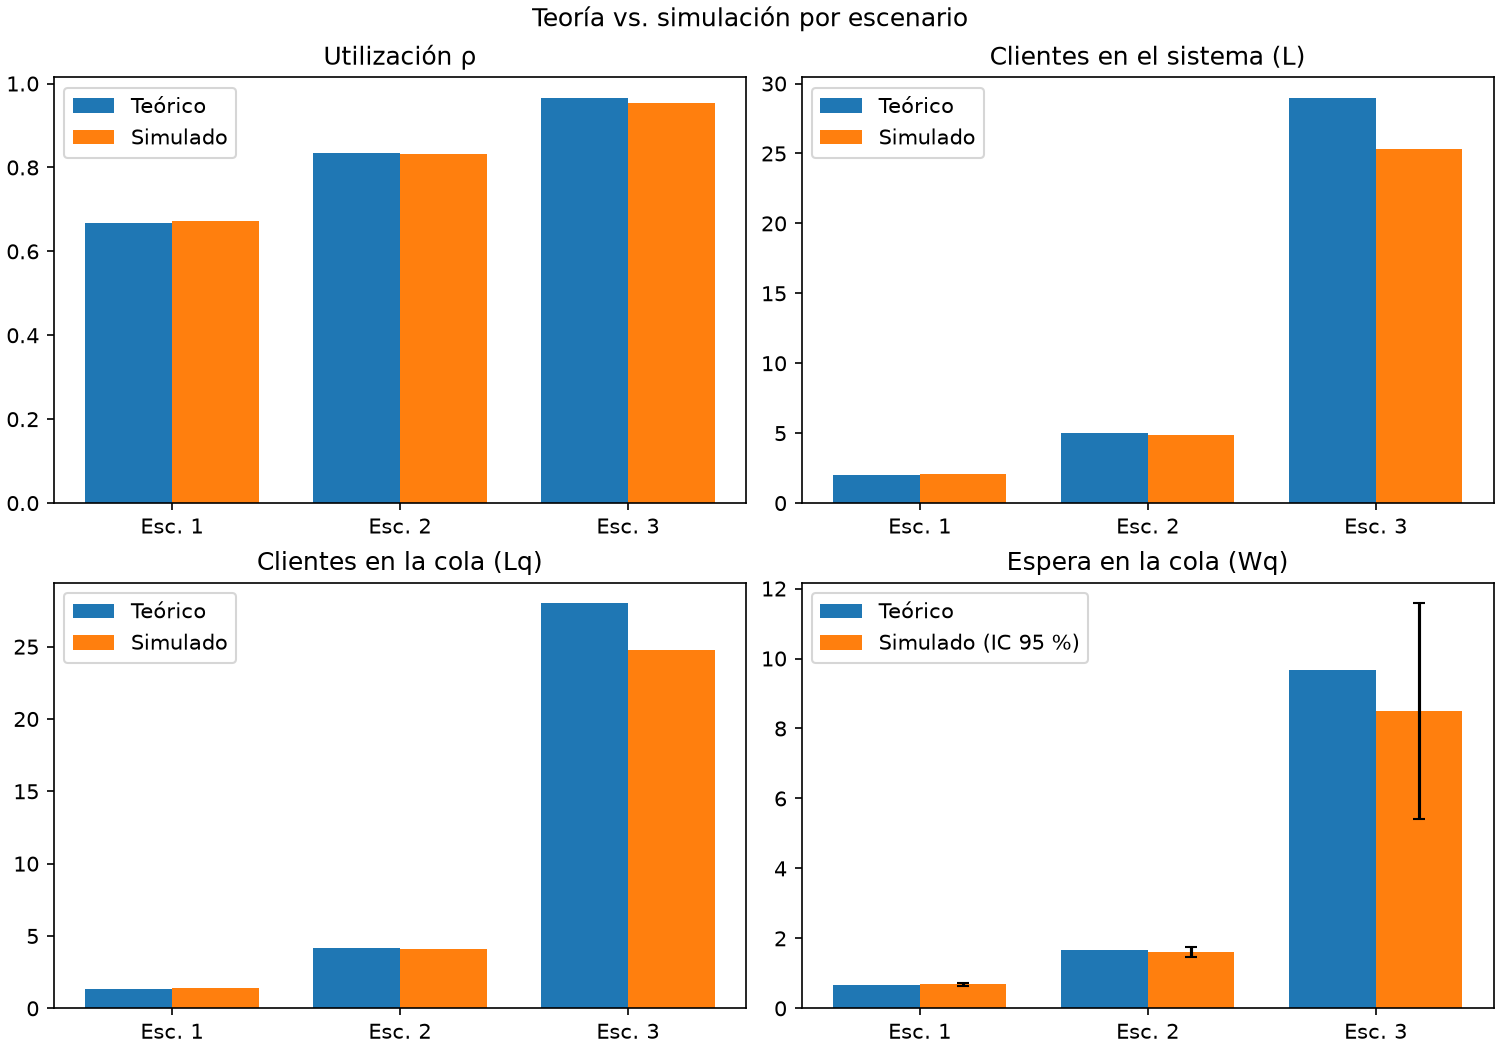
\includegraphics[width=\textwidth]{figures/teoria_vs_simulacion.png}
\caption{Comparación teoría vs.\ simulación por escenario. El intervalo de confianza
del panel $W_q$ es ancho en el escenario 3 porque $\rho \to 1$: la espera se vuelve muy
variable, pero la teoría sigue dentro del rango.}
\label{fig:teoria}
\end{figure}

La Figura~\ref{fig:comparacion} muestra el crecimiento de la espera y de la cola en
función de la utilización $\rho$.

\begin{figure}[h!]
\centering
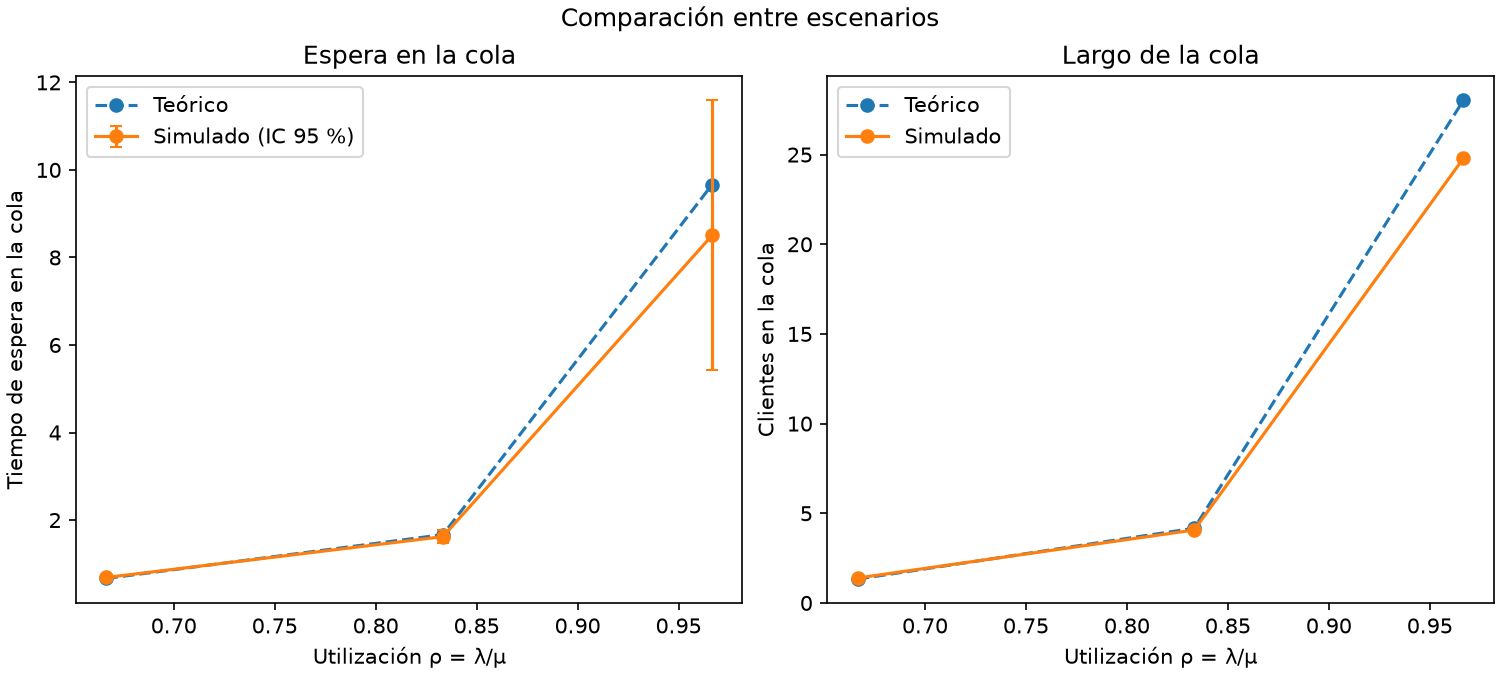
\includegraphics[width=\textwidth]{figures/comparacion_escenarios.png}
\caption{Espera en la cola y largo de la cola en función de $\rho$. El crecimiento es
marcadamente no lineal: al pasar de $\rho = 0{,}667$ a $\rho = 0{,}967$, la espera
simulada crece más de doce veces.}
\label{fig:comparacion}
\end{figure}

La Figura~\ref{fig:esc3} muestra la evolución temporal de la cola y los tiempos de espera
de cada cliente en el escenario más exigente.

\begin{figure}[h!]
\centering
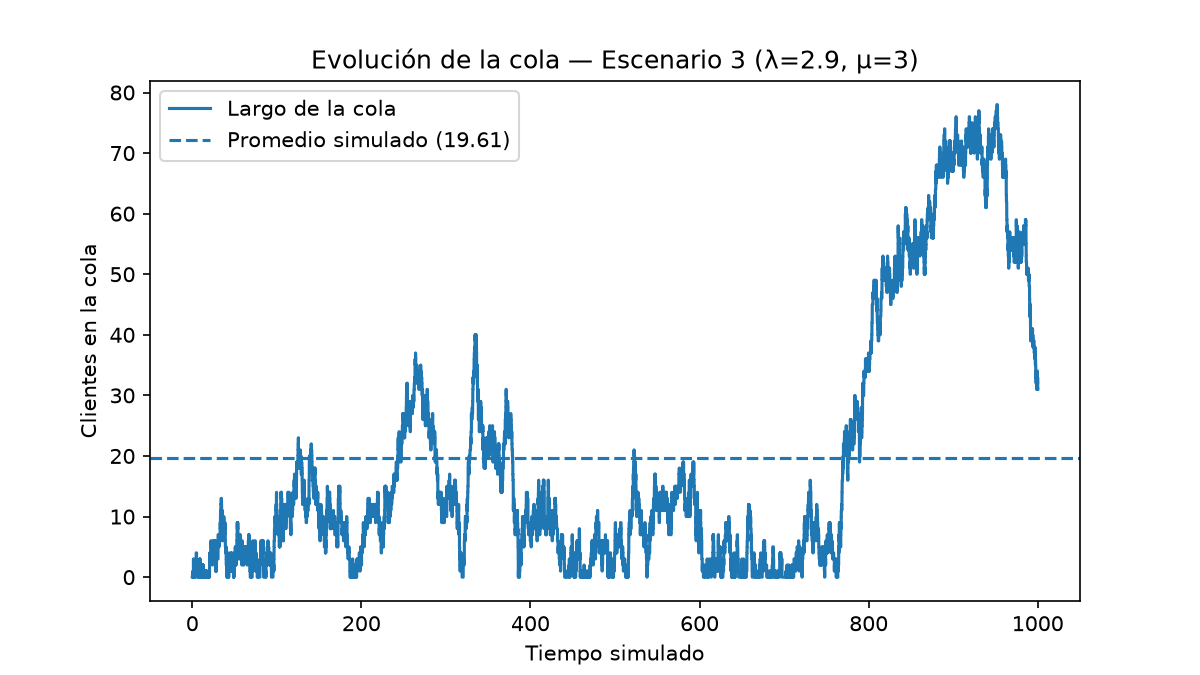
\includegraphics[width=0.49\textwidth]{figures/escenario_3_cola.png}
\hfill
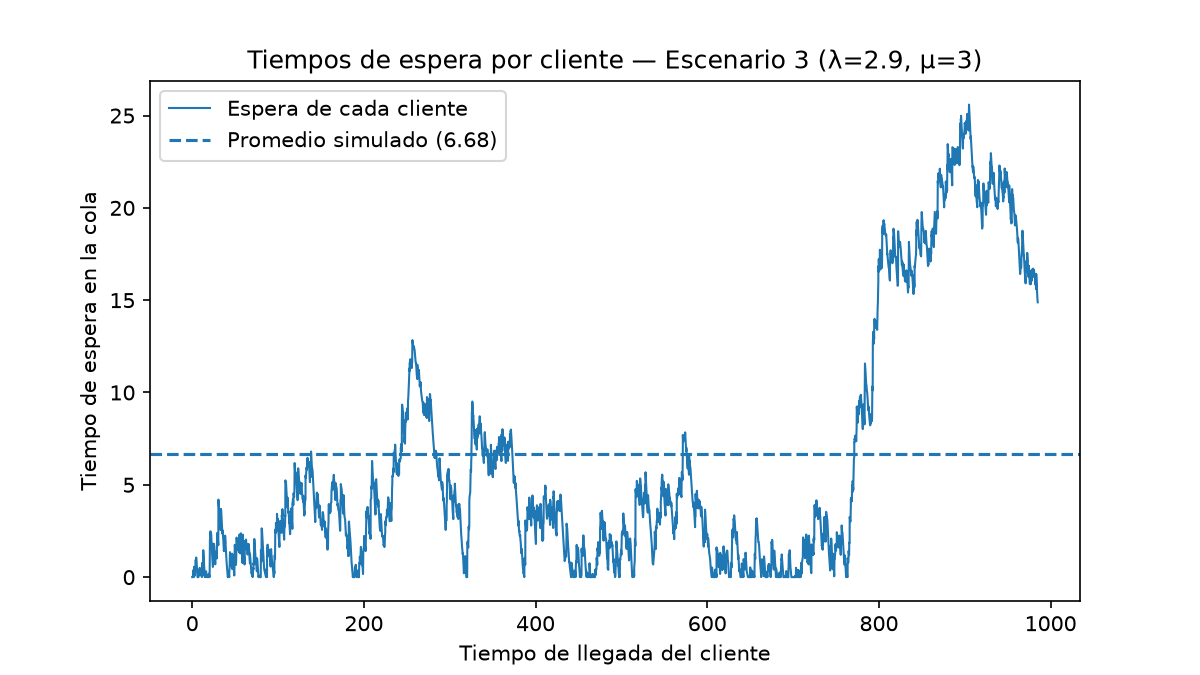
\includegraphics[width=0.49\textwidth]{figures/escenario_3_espera.png}
\caption{Escenario 3 ($\lambda = 2{,}9$, $\rho = 0{,}967$): evolución de la cola y
tiempos de espera por cliente. La cola alcanza valores altos de forma sostenida y los
tiempos de espera presentan una dispersión mucho mayor que en los escenarios 1 y 2.}
\label{fig:esc3}
\end{figure}

Las figuras equivalentes de los escenarios 1 y 2 están en
\texttt{reports/figures/} y se regeneran con el mismo comando.

\section{Análisis de Resultados}

\subsection{Comportamiento del sistema según la guía}

La guía anticipa que \emph{cuando $\lambda$ se aproxima a $\mu$, aumentan el tiempo de
espera y el tamaño de la cola, debido a que el servidor trabaja cerca de su capacidad
máxima}. Los resultados confirman ese comportamiento en las dos direcciones:

\begin{itemize}
    \item La utilización teórica crece de $0{,}667$ a $0{,}833$ y luego a $0{,}967$, y la
    utilización \emph{medida} en la simulación la acompaña ($0{,}673$, $0{,}833$ y
    $0{,}953$).
    \item El tiempo de espera simulado pasa de $0{,}69$ a $1{,}62$ y luego a $8{,}51$
    unidades, es decir un factor de más de doce entre el primer y el último escenario.
    La cola promedio simulada pasa de $1{,}39$ a $4{,}07$ y luego a $24{,}79$ clientes.
\end{itemize}

El crecimiento no es lineal sino acelerado: pasar de $\rho = 0{,}667$ a $\rho = 0{,}833$
casi duplica la espera, mientras que pasar de $\rho = 0{,}833$ a $\rho = 0{,}967$ la
multiplica por más de cinco. Esto es exactamente lo que predicen las fórmulas, donde
$W_q$ diverge cuando $\lambda \to \mu$.

\subsection{Por qué lo simulado no coincide exactamente con lo teórico}

Esta es la pregunta de control número 9 y merece una respuesta medida en lugar de una
explicación genérica. Hay cuatro razones, y las cuantificamos con nuestros datos.

\begin{enumerate}
    \item \textbf{La teoría describe el largo plazo; la simulación mide una muestra.}
    Las fórmulas $L$, $L_q$, $W$ y $W_q$ son los valores esperados del sistema en estado
    estacionario, es decir el límite cuando el tiempo simulado tiende a infinito. Una
    corrida de duración finita devuelve una estimación con varianza.

    \item \textbf{El error disminuye al alargar la corrida.} Repitiendo el escenario 1 con
    horizontes crecientes, el error relativo de $W_q$ baja de $12{,}9$\,\% con
    $\text{sim\_time} = 500$ a $5{,}7$\,\% con $2000$, $2{,}5$\,\% con $10\,000$ y
    $1{,}6$\,\% con $50\,000$. Que el error tienda a cero al aumentar la muestra es la
    firma de un estimador \emph{consistente}: el simulador converge a la teoría, no se
    desvía de ella.

    \item \textbf{Cerca de la saturación la varianza explota.} Este es el punto más
    importante y el que explica la diferencia entre el escenario 3 y los otros dos. Con
    $\rho = 0{,}967$ el tiempo de espera tiene una distribución de \emph{cola pesada}:
    la mayoría de los clientes espera poco, pero unos pocos esperan muchísimo, y esos
    pocos casos arrastran el promedio de toda la corrida. Una corrida individual de ese
    escenario puede desviarse hasta un 74\,\% de la teoría, y sin embargo la media de 30
    réplicas se reduce a un $12$\,\% y el intervalo de confianza contiene al valor
    teórico. La desviación grande de una corrida aislada \textbf{no es un error del
    simulador}: es la naturaleza del sistema cerca de la saturación.

    \item \textbf{La ley de Little se cumple en los resultados simulados.} Como
    comprobación interna independiente de las fórmulas del modelo, verificamos
    $L = \lambda \cdot W$ sobre las salidas de la simulación: el desvío es inferior al
    $0{,}9$\,\% en los tres escenarios. Si el registro de tiempos o el orden FIFO
    estuvieran mal implementados, esta relación no se cumpliría.
\end{enumerate}

Por todo lo anterior, el procedimiento correcto no es comparar una corrida contra la
teoría, sino comparar \textbf{el promedio de varias réplicas} y verificar si la teoría
cae dentro del intervalo de confianza. Eso es lo que hace la Tabla~\ref{tab:intervalos},
y el resultado es que cae en los tres casos.

\section{Preguntas de Control}

\begin{enumerate}
    \item \textbf{\textquestiondown{}Qué representa el modelo M/M/1?}
    Es un sistema de líneas de espera con un único servidor. La notación de Kendall
    describe sus tres características: la primera \emph{M} indica que las llegadas
    siguen un proceso de Poisson (tiempos entre llegadas exponenciales), la segunda
    \emph{M} que los tiempos de servicio son exponenciales, y el \emph{1} que hay un
    solo servidor. Los clientes se atienden en orden FIFO. En este trabajo los tres
    escenarios son M/M/1 con $\mu = 3{,}0$ y $\lambda$ creciente.

    \item \textbf{\textquestiondown{}Qué representan $\lambda$ y $\mu$?}
    $\lambda$ es la tasa promedio de llegada: la cantidad de clientes que llegan por
    unidad de tiempo. $\mu$ es la tasa promedio de servicio: la cantidad de clientes que
    el servidor puede atender por unidad de tiempo si nunca le falta trabajo. Sus
    recíprocos son los tiempos promedio: $1/\lambda$ es el tiempo medio entre llegadas y
    $1/\mu$ el tiempo medio de servicio. Con $\mu = 3{,}0$ el servicio promedio dura
    $1/3$ de unidad de tiempo; con $\lambda = 2{,}0$ llega un cliente cada $0{,}5$
    unidades en promedio.

    \item \textbf{\textquestiondown{}Por qué debe cumplirse $\lambda < \mu$ para que el sistema sea estable?}
    Porque la cola solo se vacía al ritmo al que el servidor atiende. Si llegan clientes
    más rápido de lo que se los puede atender, el trabajo pendiente se acumula sin
    límite y la cola crece indefinidamente. La condición equivale a $\rho = \lambda/\mu <
    1$: el servidor debe tener capacidad sobrante. Si $\lambda \geq \mu$ el sistema no
    alcanza un estado estacionario y $L$, $L_q$, $W$ y $W_q$ no tienen valor finito. En
    el programa esta condición se verifica antes de simular y, si no se cumple, se
    informa \texttt{El sistema no es estable} sin ejecutar la simulación.

    \item \textbf{\textquestiondown{}Qué significa la utilización $\rho$?}
    Es la fracción del tiempo que el servidor está ocupado, $\rho = \lambda/\mu$. Su
    valor está entre 0 y 1 para un sistema estable. En la simulación se mide como el
    tiempo total de servicio efectivo dividido por el tiempo observado, y coincide con la
    teoría: $0{,}673$, $0{,}833$ y $0{,}953$ medidos contra $0{,}667$, $0{,}833$ y
    $0{,}967$ teóricos. Un $\rho$ cercano a 1 indica un servidor casi saturado, y es ahí
    donde los tiempos de espera se disparan.

    \item \textbf{\textquestiondown{}Cuál es la diferencia entre $W$ y $W_q$?}
    $W$ es el tiempo total que un cliente permanece en el sistema, desde que llega hasta
    que termina de ser atendido. $W_q$ es solo el tiempo que espera en la cola antes de
    que empiece su servicio. La relación es $W = W_q + 1/\mu$. En nuestros resultados del
    escenario 1: la espera simulada es $0{,}6885$ y el tiempo en el sistema es
    $1{,}0336$, y la diferencia $0{,}3451$ es aproximadamente $1/\mu = 0{,}3333$, el
    tiempo medio de servicio. La diferencia entre ambas medidas es constante: es el
    servicio, no la congestión.

    \item \textbf{\textquestiondown{}Cuál es la diferencia entre $L$ y $L_q$?}
    $L$ es la cantidad promedio de clientes en el sistema, contando tanto los que esperan
    como el que está siendo atendido. $L_q$ cuenta solo los que esperan en la cola. La
    relación es $L = L_q + \rho$, porque el cliente en servicio aporta una fracción
    $\rho$ del tiempo. En el escenario 1: $L = 2{,}0639$ y $L_q = 1{,}3921$, y la
    diferencia $0{,}6718$ coincide con la utilización medida $0{,}6732$: es el cliente
    que ocupa el servidor.

    \item \textbf{\textquestiondown{}Por qué SimPy utiliza una distribución exponencial para generar los tiempos?}
    Porque es la distribución que corresponde al supuesto de llegadas de Poisson. En un
    proceso de Poisson los tiempos \emph{entre} eventos consecutivos se distribuyen
    exponencialmente, de modo que generar intervalos exponenciales es la forma de
    construir llegadas de Poisson. Además, la exponencial es la única distribución
    continua \emph{sin memoria}: la probabilidad de que un cliente llegue en el próximo
    instante no depende de cuánto tiempo se lleva esperando desde la llegada anterior.
    Esa propiedad es lo que hace que el estado del sistema dependa solo de la cantidad de
    clientes presentes y no del historial, y es lo que permite deducir las fórmulas
    cerradas de $L$, $L_q$, $W$ y $W_q$. Si los tiempos siguieran otra distribución, el
    modelo dejaría de ser M/M/1.

    \item \textbf{\textquestiondown{}Qué sucede con la cola cuando $\lambda$ se aproxima a $\mu$?}
    La cola y el tiempo de espera crecen de forma acelerada, no proporcional. Al acercarse
    $\lambda$ a $\mu$, $\rho$ tiende a 1 y el denominador $\mu - \lambda$ de las fórmulas
    tiende a cero, de modo que $L$, $L_q$, $W$ y $W_q$ crecen sin límite. Nuestros datos
    lo muestran: la cola promedio simulada pasa de $1{,}39$ clientes con $\rho = 0{,}667$
    a $4{,}07$ con $\rho = 0{,}833$ y a $24{,}79$ con $\rho = 0{,}967$, mientras la espera
    pasa de $0{,}69$ a $1{,}62$ y a $8{,}51$. El servidor trabaja casi todo el tiempo y
    cualquier ráfaga de llegadas se traduce directamente en cola.

    \item \textbf{\textquestiondown{}Por qué los resultados simulados pueden ser diferentes de los resultados teóricos?}
    Porque la teoría da el valor esperado en estado estacionario y la simulación mide una
    muestra finita, que tiene varianza. Verificamos tres hechos con nuestros datos: el
    error disminuye al alargar la corrida (de $12{,}9$\,\% a $1{,}6$\,\% al pasar de 500 a
    50\,000 unidades), la ley de Little se cumple sobre las salidas simuladas con menos de
    $0{,}9$\,\% de desvío, y el valor teórico cae \emph{dentro} del intervalo de confianza
    al 95\,\% en los tres escenarios. Cerca de la saturación ($\rho = 0{,}967$) la
    dispersión es muy grande porque la espera tiene cola pesada: una corrida individual
    puede desviarse hasta un 74\,\% y aun así el modelo estar bien implementado. Por eso el
    informe compara promedios de 30 réplicas con su intervalo de confianza, y no corridas
    individuales.

    \item \textbf{\textquestiondown{}Qué ocurriría si $\lambda$ fuera mayor que $\mu$?}
    El sistema sería inestable: como llegan clientes más rápido de lo que se los atiende,
    el trabajo pendiente se acumula y la cola crece indefinidamente, sin alcanzar nunca un
    estado estacionario. $\rho$ sería mayor que 1, lo que significa que el servidor
    necesitaría más tiempo de servicio del que dispone, y las medidas $L$, $L_q$, $W$ y
    $W_q$ no tendrían valor finito. El programa detecta esta situación y responde
    \texttt{El sistema no es estable} con un código de salida distinto de cero, sin
    ejecutar la simulación. Para atender esa demanda habría que agregar servidores
    (un modelo M/M/c) o aumentar la capacidad de servicio.
\end{enumerate}

\section{Conclusiones}

\begin{enumerate}
    \item \emph{Sobre implementar un modelo M/M/1 con SimPy.} El sistema quedó
    implementado y funcionando: un servidor de capacidad 1, llegadas exponenciales,
    servicio exponencial, atención FIFO y registro por cliente. La simulación de los tres
    escenarios de la guía se reproduce con un solo comando, de forma determinista, gracias
    a que las semillas se derivan de una semilla base. Se registran por cliente el instante
    de llegada, el inicio y fin de servicio, el tiempo de espera y el tiempo de servicio,
    y se conserva la traza temporal de la cola.

    \item \emph{Sobre calcular las métricas teóricas.} Las cinco medidas del modelo
    ($\rho$, $L$, $L_q$, $W$ y $W_q$) quedaron implementadas según las fórmulas de la guía
    y se usaron como \emph{oráculo} para verificar el simulador. Vale registrar que la
    guía imprime $\rho = \mu/\lambda$, incoherente con su propia condición de estabilidad;
    se usó la definición correcta $\rho = \lambda/\mu$, sin la cual los tres escenarios
    propios de la guía darían un servidor saturado y las demás métricas carecerían de
    valor.

    \item \emph{Sobre comparar teoría y simulación.} La comparación se hizo entre la
    teoría y el promedio de 30 réplicas por escenario, con su intervalo de confianza al
    95\,\% y el error relativo de cada medida. El resultado central es que \textbf{en los
    tres escenarios el valor teórico cae dentro del intervalo simulado}, con errores
    relativos entre $2{,}1$\,\% y $12{,}7$\,\%. Queda además caracterizado el efecto que
    predice la guía: conforme $\lambda$ se aproxima a $\mu$, la utilización sube y tanto
    la espera como la cola crecen de forma acelerada, más de doce veces entre el primer y
    el último escenario. La principal limitación metodológica encontrada es que cerca de
    la saturación una corrida aislada no es evidencia suficiente y hay que reportar la
    incertidumbre; hacia allí apunta el uso del intervalo de confianza.
\end{enumerate}

\section{Demostración}

El video de demostración muestra la ejecución del sistema desde la línea de comandos:
la corrida de los tres escenarios, la generación de la tabla comparativa y de las
figuras, y la animación de la evolución de la cola.

\pendiente{enlace al video de demostración y a la animación
(\texttt{cola.mp4})}

\section{Bibliografía}

\nocite{*}
\bibliographystyle{plain}
\bibliography{referencias}

\end{document}
